
\documentclass{sig-alternate}
\usepackage{color}
\usepackage[colorinlistoftodos]{todonotes}
\usepackage{listings}
%\usepackage{float}


%%%%% Uncomment the following line and comment out the previous one
%%%%% to remove all comments
%%%%% NOTE: comments still occupy a line even if invisible;
%%%%% Don't write them as a separate paragraph
%\newcommand{\mycomment}[1]{}

\begin{document}

% --- Author Metadata here ---
\conferenceinfo{UMM CSci Senior Seminar Conference, April 2016}{Morris, MN}

\title{Security of Near Field Communication:\break Does My Phone Need A Tinfoil Hat?}

\numberofauthors{1}

\author{
\alignauthor
Thomas Harren\\
	\affaddr{Division of Science and Mathematics}\\
	\affaddr{University of Minnesota, Morris}\\
	\affaddr{Morris, Minnesota, USA 56267}\\
	\email{harre096@morris.umn.edu}
}

\maketitle
\begin{abstract}
Near Field Communication (NFC) is a technology that is rapidly growing in popularity and is becoming even more common due to the advent of mobile payment systems. Near Field Communication  is built upon High Frequency Radio Frequency Identification technology, more commonly known as HF RFID. NFC is a flexible communication technology, but it is not inherently secure. The limited range of NFC offers some security, but data transmitted using NFC is still vulnerable to various attacks. As a result, measures to ensure confidentiality, integrity, and authentication need to be implemented as an extension of NFC. Moreover, if the data transmitted from a peer is malicious, a hardware-based firewall may be a good way to defend your NFC capable device. One proposed technology is a device-independent security method, a metaphorical tin foil hat, that could defend against current and evolving attacks on NFC enabled devices.
\end{abstract}

\keywords{Near Field Communication (NFC), Payments, Ticketing, Mass Transit, Security, Privacy, Jamming}

\section{Introduction}
\label{sec:introduction}
Near Field Communication is a technology that is rapidly growing in popularity and is becoming even more common due to the advent of mobile payment systems. \textit{Near Field Communication} (NFC) is built upon High Frequency Radio Frequency Identification technology, more commonly known as HF RFID. NFC is restricted to a shorter range than RFID and offers interactive communication method between devices that have both passive and active components. An NFC connection can be set up quickly and connectivity does not require line of sight. Uses of NFC technologies are being rapidly developed to be used in payment systems and in other applications~\cite{Gum2013}.

NFC is a flexible communication technology, but it is not inherently secure. The limited range of NFC may make attacks more difficult, but data transmitted using NFC is still vulnerable. For sensitive data, measures to ensure confidentiality, integrity, and authentication need to be implemented as an extension of NFC~\cite{CC2016}. One proposed technology offers a flexible hardware firewall that may be an effective way to block data transfers with malicious peers~\cite{Gum2013}.

In this paper, we focus on security and applications of NFC regarding payments and ticketing. First, we describe the foundations of Near Field Communication in Section~\ref{sec:background}. Then, we discuss security in three different NFC contexts: contactless credit cards, mobile ticketing applications, and physical NFC security.
In Section~\ref{sec:creditCard}, we highlight several viable attacks on
contactless credit cards and summarize a proposed solution.
In Section~\ref{sec:mobile}, we discuss a prospective application for the richer NFC communication, using mobile phones for mass transit ticketing. Three implementations of mobile ticketing are introduced, prototyped, and critiqued by three Nokia researchers, each balancing security and transaction time in a unique way.
This leads to a discussion of the EnGarde shield in Section~\ref{sec:enGarde}. Commercial payment systems such as Apple Pay and Android Pay are bringing NFC to mobile phones, which could introduce security risks in both payment and non-payment applications of NFC. The proposed device utilizes an independent, hardware-based firewall which may be a viable way to defend against more general threats.


\section{Background}
\label{sec:background}
In this section, we provide an overview of Near Field Communication and properties of its physical operation.  We first discuss RFID technology, the parent technology of NFC. Next, we discuss additional features specific to the NFC standard.
%Since this paper emphasizes NFC in the context of payments, we will briefly describe the current status of the payment industry.
Finally, we highlight the need for explicit security when using NFC.

\subsection{Elements of HF RFID: Tags \& Readers}
\label{sec:activePassive}

NFC is a wireless communication standard that is based on, and fully compatible with, the HF RFID (high frequency radio-frequency identification) standard~\cite{Gum2013}. At a fundamental level, this means that communication happens between tags and readers.

A \textit{tag} is composed of an integrated circuit and an antenna. A tag is capable of storing a unique ID and a limited amount of data, which can be read/write or read only. RFID tags can be actively powered, battery assisted, or passively powered. A passive tag relies exclusively on energy induced into the tag's antenna coil. Since passive tags require no built in power source, they are the least expensive and smallest RFID tags. While the tag is powered, it can use its antenna coil to relay its internal information back to the other party.~\cite{wiki:RFID}

A \textit{reader} is a device used to power and interrogate RFID tags. A reader emits an electromagnetic field in order to power nearby tags. Before initiating communication, the reader runs a discovery protocol. If multiple tags respond, the reader uses its collision avoidance protocol to establish communication with a single tag using one tag's unique ID. The tag and the reader then communicate by taking turns sending and receiving messages.~\cite{Gum2013}

A standard RFID reader-tag interaction is illustrated in Figure~\ref{fig:rfid}. Both the reader and tag have antenna coils tuned to the standard 13.56MHz frequency. When the reader generates an electromagnetic field, the reader and the tag are coupled, and power is induced into the tag's antenna coil; this energy transfer is similar to that found in electrical transformers. The tag then converts the AC voltage it receives into DC voltage in order to power the tag's circuit. The electromagnetic field of this frequency is able to power a tag within a range of a few centimeters. According to Gummeson et al, the communication distance can be increased up to 1 meter if larger, higher powered readers are used.~\cite{Gum2013}


%\textcolor{red}{Communication happens using amplitude modulation (AM) from the reader to the tag. Then the tag uses a parallel resistor to modulate the load across the tag coil. Varying the load leads to varying the current and voltage that the reader coil receives. Various encoding schemes are then used to send messages in this way.}
\begin{figure}
\centering
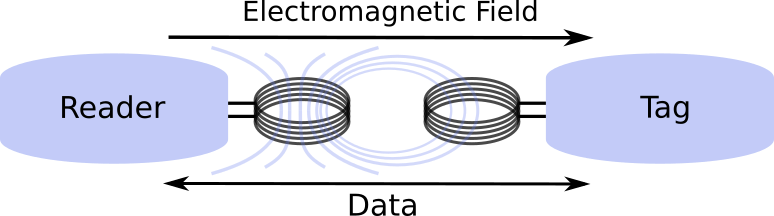
\psfig{file=figures/emitterAndTagWide.png,width=3in,natwidth=700,natheight=189}
\caption{Readers and tags interact with each other using antenna coils and electromagnetic induction.}
%Neat diagram from http://www.mouser.com/applications/rfid-nfc-introduction/ and another at http://electronicdesign.com/communications/nfcrfid-ripe-application-expansion
\label{fig:rfid}
\end{figure}

\subsection{NFC on Mobile Phones}
\label{sec:nfcOnPhones}
Near field communication also has features that extend beyond the HF RFID specification. In particular, an NFC enabled mobile phone can function in several unique modes:
\vspace{2mm}\newline
\textbf{Phone acting as a reader:}
In this mode, a mobile phone functions as an RFID tag reader. Touching a phone to a tag mounted to a map, for example, could send the phone a hyperlink to a informational page.~\cite{staticDynamicDisplays}
\vspace{2mm}\newline
\textbf{Phone emulating a tag:}
A mobile phone can also function as if it was a passive tag. This mode can be effectively used even when the phone is not powered, because power is induced by an NFC reader. Mobile payments and ticketing applications would tend toward this interaction mode.~\cite{Gum2013}
\vspace{2mm}\newline
\textbf{Phone acting as a peer:}
When two compatible devices are capable of switching between reader and tag emulation mode, they can communicate directly over NFC in a peer-to-peer manner. Peer-to-peer mode offers the highest communication throughput and can be used to implement stronger security~\cite{Ticket2011} or to coordinate mobile file transfers.~\cite{Gum2013}

\subsection{Security for NFC}
\label{sec:backgroundSecurity}
NFC is a flexible communication technology, but it is not inherently secure. The limited range of NFC makes attacks more difficult, but data transmitted using NFC is still vulnerable to attacks, as discussed in Section~\ref{sec:attacks}. As a result, measures to ensure confidentiality, integrity, and authentication need to implemented as an extension of NFC. Maintaining security of NFC is the main focus of this paper.~\cite{CC2016}



%%%%%%%%%%%%%%%%%%%%%%%%%%%%%%%%%%%%%%%%%%%%%%%%%%%%%%%%%%%%%%%%
\section{Contactless Credit Cards}
\label{sec:creditCard}
In this section, we look at the usage of passively powered NFC tags installed into  credit cards and some related security concerns. Jensen, Gouda, and Qiu's~\cite{CC2016} work is the focus of this section. They describe several effective contactless credit cards attacks and propose a security protocol to defend against these attacks. Since their security protocol must run on a passively powered NFC chips embedded in credit card, it is composed of computational inexpensive primitives including pre-computed hashes, indexing and XOR operations.~\cite{CC2016}


\subsection{Current Credit Card Protocol}
\label{sec:currentCC}
As background, we will describe the current credit card protocol used for NFC transactions. The current protocol transmits card data in plain text, but does offer some level of security by merit of the iCVV. A dynamic card verification value or \textit{iCVV} is a single use value that a contactless credit card generates for each transaction~\cite{wiki:iCVV}. The iCVV is returned from a pesudo-random sequence using a seed known only to that specific credit card and the issuing bank. At the time of authorization, the bank checks that the iCVV received is one of the expected values in that card's iCVV sequence. The four phases of the credit card protocol used for NFC transactions are illustrated in Figure~\ref{fig:currentCC}, and will now be described.

\begin{figure}
\centering
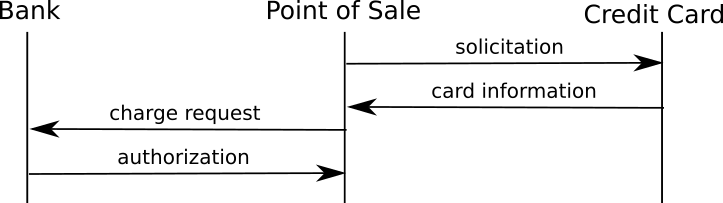
\psfig{file=figures/CCcurrent.png,width=3in,natwidth=700,natheight=189}
\caption{The basic steps executed in an NFC transaction using the current credit card protocol.
\cite{CC2016}}
\label{fig:currentCC}
\end{figure}

In the first phase, called \textit{solicitation}, the point-of-sale and the credit card exchange several messages in a static manner. In this phase, both parties share general information about themselves. For example, a card may identify itself as \texttt{VISA CREDIT}.

In the second phase, \textit{card information} is sent from the card to the point-of-sale. The card information is composed of the credit card number, the credit card's expiration date, the iCVV, and the name of the bank that issued the card.

The point-of-sale then sends the card information to the bank in the third phase, called the \textit{charge request}. The credit card's number and expiration date, along with the iCVV and the dollar amount charged, are sent to the specified bank.

The final phase is called \textit{authorization} and only occurs if the bank deems the card information valid. Banks may also perform other checks based on the transaction's physical location or other factors.


\subsection{Credit Card Attacks}
\label{sec:attacks}
The following attacks on NFC transactions may vary slightly, but each method ultimately exposes sensitive card information. The first three attacks can be accomplished with merely a NFC compatible mobile phone and some additional, inexpensive hardware. The final attack, compromised point-of-sale, points out a more general weakness about the implementation of the current protocol.
\vspace{2mm}\newline
\noindent\textbf{Eavesdropping:}
In this attack, a malicious party is able to capture sensitive data by listening in on the first two phases of a transaction. Thus, the card number, expiration data, iCVV, and bank name are gleaned by the malicious party. The iCVV cannot be used again, but the other information may already be enough to make a fraudulent purchase.

\begin{figure}
\centering
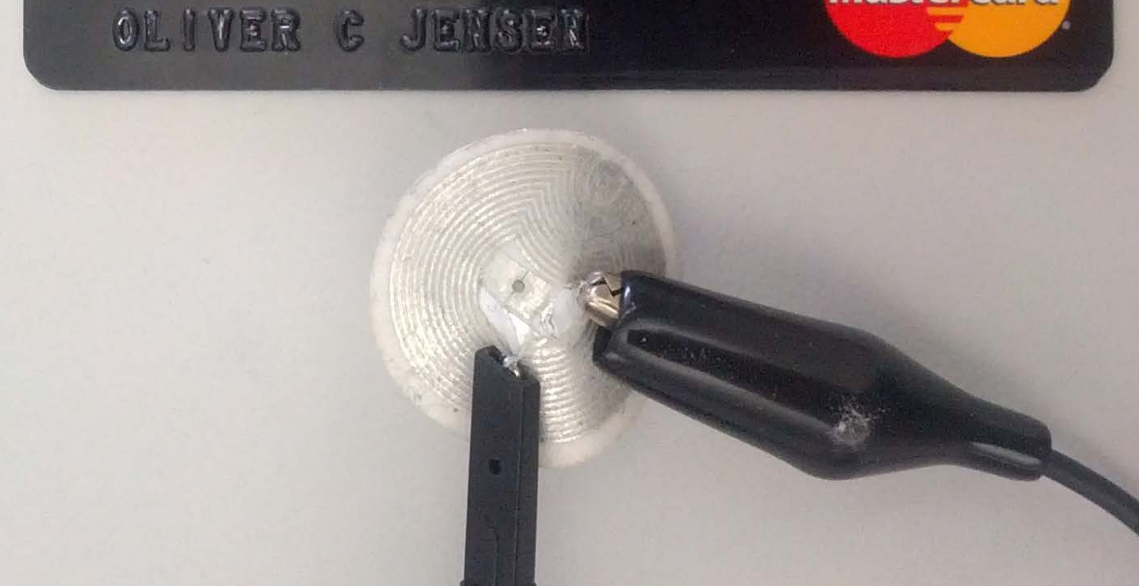
\psfig{file=figures/eavesdroppingAntenna.png,width=3in,natwidth=700,natheight=189}
\caption{A small eavesdropping antenna~\cite{CC2016} (card for scale)}
\label{fig:antenna}
\end{figure}

The researchers demonstrated the feasibility of this attack by building an eavesdropper using an NFC tag and an inexpensive radio. The very small, easy concealable eavesdropping antenna is shown in Figure~\ref{fig:antenna}. The antenna could be mounted or held within the range of a contactless NFC credit card terminal.
\vspace{2mm}\newline
\noindent\textbf{Skimming:}
In this attack, illustrated in Figure~\ref{fig:skim}, a skimmer gains a victim's credit card information, including a single usable iCVV, by masquerading as a point-of-sale. After the skimmer has captured this data, it can replay the credit card information to a genuine point-of-sale to perform an illegitimate purchase on behalf of the victim.

Surprisingly, this attack can be carried out by simply installing an Android application called \textit{NFCProxy}.\footnote{\textit{NFCProxy} was presented at DefCon 20 and can be downloaded at: https://sourceforge.net/projects/nfcproxy/~\cite{CC2016}}
Using \textit{NFCProxy}, any NFC enabled Android device can skim information from a contactless credit card which can later be used to make a purchase. To make subsequent purchases, the attack can be repeated to obtain new iCVVs.
\begin{figure}
\centering
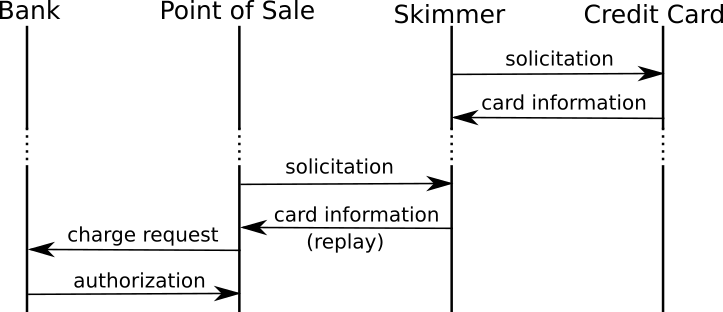
\psfig{file=figures/CCskim.png,width=3in,natwidth=700,natheight=189}
\caption{Skimmers capture, then replay, card data.~\cite{CC2016}}
\label{fig:skim}
\end{figure}
\vspace{2mm}\newline
\noindent\textbf{Relay Attacks:}
In this attack, two devices work in concert to rapidly carry out the skimming attack. Skimmed data is sent to an accomplice using a non-NFC communication channel such as wireless LAN. Once the accomplice receives the card data, they can replay it at a point of sale using their own phone.
\vspace{2mm}\newline
\noindent\textbf{Compromised Point-of-Sale:}
This attack points out that since point-of-sale devices learn enough information to allow multiple charges, the point-of-sale is a natural target. If a point-of-sale is compromised, transaction becomes accessible to malicious parties. Jensen, Gouda, and Qiu list several merchants that have recently had their point-of-sale systems compromised including Target, Home Depot, and SuperValu stores.

\subsection{Proposed Secure Credit Card Protocol}
To address these security concerns, Jensen, Gouda, and Qiu have proposed a secure protocol which shares the same four phases as the current credit card protocol (Figure~\ref{fig:currentCC}), but with several variations that will be described and illustrated using the Figure~\ref{fig:secureCC}.

\begin{figure}
\centering
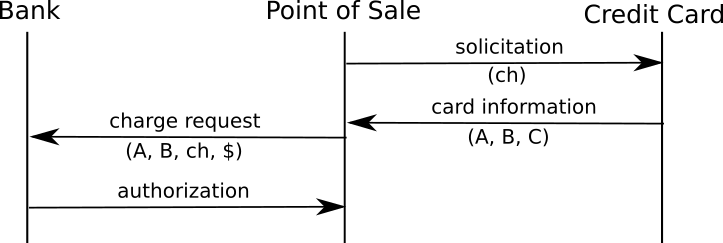
\psfig{file=figures/CCnew.png,width=3in,natwidth=700,natheight=189}
\caption{Proposed Credit Card Protocol~\cite{CC2016}}
\label{fig:secureCC}
\end{figure}

The solicitation phase now includes a random challenge (\textbf{ch}). A challenge is a piece of random data that each terminal will generate for each new transaction. That challenge acts as an authentication tool and will be used by the credit card when building its response. After receiving some basic information and the challenge, the credit card responds by sending the card information in three distinct pieces:
\begin{itemize}
  \item \textbf{A}: \textbf{\textit{UUID}}, a Universally Unique Identifier that is used to identify the credit card. The UUID is static.
  \item \textbf{B}: \textit{\textbf{H(info, ch, iCVV})} is used to authenticate the card's identity. Notice that the sensitive info, including the card number and expiration date, will not be transmitted in plain text. The details of the function H are described below.
  \item \textbf{C}: \textbf{\textit{bank name}} is used to route the charge request.
  \end{itemize}
Upon receiving all three parts of the card information, the point-of-sale simply forwards the UUID (\textit{A}) and the authentication (\textit{B}) to the bank (\textit{C}) learning nothing about the actual card data. The challenge (\textit{ch}) is also sent so that the bank will have all of the pieces necessary to generate the authentication value and check for validity by matching it to \textit{B}. The bank will also receive the charge amount \textit{\$}.

Finally, the bank uses the \textit{UUID} to look up official card data. Then the bank uses  the H function with its own copy of the customer information and the challenge (\textit{ch}) to create \textit{B\begin{tiny}bank\end{tiny}}. If \textit{B\begin{tiny}bank\end{tiny}} = \textit{B}, then the bank considers the card data valid and authorizes the charge.
\vspace{2mm}\newline
\noindent\textbf{Requirements of function H:} H works like a hash function. It uses several inputs to creates an output that is indistinguishable from random and cannot be used to derive the original inputs. A hash output can only be verified by using creating a new copy of the output; if the inputs were the same, then the outputs will match.
% So long as \textit{B}, the output of H function, appears random, no sensitive information can be learned from an eavesdropping attack. Also, when a skimming or relay attacker collects \textit{ch} and \textit{B} and attempts to replay the card information, it will not be able to calculate the new output value \textit{B$'$} when given the new challenge \textit{ch$'$}.
Here is the pseudo-code for the function H:

\begin{lstlisting}
function G(info, ch):
  const bgh = <bank-generated hash>
  result = empty list of bits
  for each of the n bits of ch:
    if the nth bit of ch is 1:
      append nth bit of bgh to result
  return result

function H(info, ch, iCVV):
  x = G(info, ch)
  return (x XOR iCVV)
\end{lstlisting}

In summary, G composes a binary string $x$ by setting values to 1 at indexes where that value in the challenge matches the value of $bgh$. Note that the value of $bgh$ is a constant generated by the bank, using card info, and is only computed when the credit card is manufactured. The value $x$ is then combined with the credit card's freshly generated iCVV using XOR. This creates a value that will appear random when intercepted. Also, the value returned cannot be easily used in a replay attack as it was built using a specific challenge value from the instigating reader. Using this method, a low powered credit card can encode and transmit payment information while being protected from all of the aforementioned attacks.




\section{NFC and Mass Transit Ticketing}
\label{sec:mobile}

Mass transit systems have widely adopted contactless NFC cards for identity verification and ticketing. In this section, we focus on the work of three Nokia researchers --- Tamrakar, Ekberg, and Asokan ~\cite{Ticket2011} --- who have investigated the use of NFC-enabled mobile phones for ticketing. In their paper, they seek to achieve security while keeping transaction time below an industry recommended 300ms threshold.
They first describe the the pieces involved in building a complete identity-verification ticketing architecture. Then, three implementations of mobile ticketing are introduced, prototyped, and critiqued.~\cite{Ticket2011}

\subsection{Ticketing Architecture}
\begin{figure}
\centering
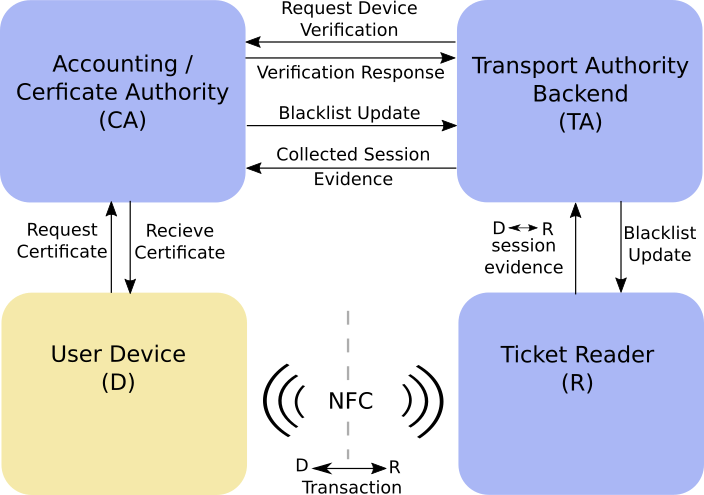
\psfig{file=figures/ticketingArch.png,width=3in,natwidth=700,natheight=189}
\caption{Proposed Ticketing Architecture~\cite{Ticket2011}}
\label{fig:ticketingArch}
\end{figure}

For NFC phones to be used for mass transit ticketing, additional infrastructure is required. An overview of the high level components and their iterations is illustrated in Figure~\ref{fig:ticketingArch}. The Accounting / Certificate Authority (CA) is a centralized entity responsible for issuing transport IDs, clearing transactions, maintaining billing information, and maintaining a blacklist. The blacklist keeps track of individuals who have been explicitly disallowed from using transit. The User Device (D) is a smartphone capable of executing cryptographic operations. D uses WLAN or a mobile data connection to attain a transport ID from CA. A ticket reader (R) is installed at each transit gate. R communicates with the D using NFC and the other entities using infrastructure. Finally, the Transport Authority Backend (TA) is an entity capable of operating all of the ticket readers and gates. In addition, the TA collects evidence from D$\leftrightarrow$R transactions for calculating fares, submits such session evidence to the CA, and queries the CA blacklist in order to distribute changes to all ticket readers.

\subsection{Security Tools}
The limited range of NFC offers some security, but data transmitted using NFC is still vulnerable to several attacks. In order to maintain secure communication, several standard security and cryptography tools will be used.
\vspace{2mm}\newline
\noindent\textbf{Trusted Hardware:}
Mobile phones are capable of doing cryptographic operations which are executed in the phone's \textit{trusted execution environment}, or TEE. Some TEEs are hardware agnostic while others extend core processing to strengthen security. In both implementations, TEEs aim to provide a secure location of sensitive data and computations.~\cite{Ticket2011}
%\vspace{2mm}\newline
%\noindent\textbf{EMV:}
%EVM is a global payment standard, developed by Europay, MasterCard, and Visa, that defines chip-based credit card standards as well as three offline data authentication techniques.~\cite{Ticket2011} Presently, EMV chip technology is being deployed as an alternative to magnetic stripe based cards in the United States. Additionally, EMV is the basis for mobile payment technologies such as Apple Pay and Android Pay.
\vspace{2mm}\newline
\textbf{Secure Communications:}
There are various methods for securing communication over an insecure channel such as NFC. In a simple symmetric key system, both parties have a secret key that is used to encrypt and decrypt messages at each end of a communication channel. This works very well, but distributing the private key to both parties can present a problem. The asymmetric key system works differently, requiring both a private key and a complementary public key. Public keys are distributed and can be used by anyone to encrypt a message that can only be decrypted by the matching private key.

In addition to messages being encrypted, they can also be authenticated and protected against modification using a \textit{signature} or \textit{message authentication code} ($MAC$). Both of these tools are similar as they use keys to generate a distinct, verifiable message based on the contents of the message body. MACs create this verifible message using a symmetric key, while signatures use an asymmetric key.\cite{crypto}

\subsection{Ticketing Protocols}
In the standard protocol, D first uses WLAN or mobile data to attain an identity \textit{certificate} from CA that is valid for several months. A certificate is a digital document containing attributes associated to the holder, in this case D, from the trusted party, the CA~\cite{crypto}. Under the D$\leftrightarrow$R transaction begins, D first receives a challenge from R.  D then sends its certificate and uses the challenge to build a signature. Once R receives and validates both the certificate and signature, checks for D on a blacklist, and opens the gate.

The drawback of using a certificate, however, lies in the large keys required by the \textit{RSA} algorithm. RSA is the chosen asymmetric cryptography system and lengthy RSA keys take substantial time to transmit over NFC.

As an alternative, the authors propose replacing the certificate with a token in Variant 1. The token is only valid for a few hours and it does not contain the large RSA key. As a result, a MAC needs to be used instead of a signature and the NFC transaction is much faster.

Variant 2 is built upon Variant 1, but uses a reversed hash chain\footnote{
A hash chain depends on some hash function that can easily generate term $t+1$ in the sequence by hashing term $t$. However, given $t$ and the hash function, $t-1$ cannot be deduced. When the hash chain is revealed in reverse, a new $t-1$ can be revealed when desired and easily verified by using the hash function to generate the known term $t$.
} to build a hybrid system that uses a long term certificate along with timely hash chain information. Revealing terms of a hash chain in reverse order is useful because it gives D a series of keys that R can validate, but other parties will not be able to predict.

\subsection{Viability Mobile Phone Ticketing}
Based on experimental measurements, Tamrakar, Ekberg, and Asokan, calculated transaction speeds for each protocol at various encryption key sizes. The results, displayed in Table~\ref{tab:speedTable}, reveal that several of the speeds are very close to or beyond the 300ms threshold. They also note that 1024 bit key size has been deprecated by EMV since 2009 and that 1152 bit keys are stated as acceptable up to 2011. Interestingly, the limited NFC data transfer speeds were found to be the biggest performance bottleneck.

\begin{table}
  \centering
  \caption{Estimated protocol speeds~\cite{Ticket2011}}
  \label{tab:speedTable}
  \begin{tabular}{c|c|c|c}
    RSA Key Size & Standard & Variant 1 & Variant 2\\
    \hline
    1024 bits & 296 ms & 164 ms & 182 ms\\
    1152 bits & 314 ms & 172 ms & 190 ms\\
    2048 bits & 482 ms & 228 ms & 246 ms\\
  \end{tabular}
\end{table}

In terms of security, the Nokia researchers grant that since users need not interact with phone to complete transactions, replay attacks are possible on all protocol variants, especially if the ticketing application is set to always-on to improve usability. Using perishable tokens or the hash chain may mitigate threats, the better user experience and accounting offered by using phones for ticketing may be worth the risk -- especially when the risk is small theft in a well-known, guarded transit station. Furthermore, contactless cards, an alternative NFC ticketing technology, does not meet performance or security needs. With these constraints in mind, the researchers contend that, although imperfect, the variant protocols appear be valid paths forward as mobile-based ticketing continues to mature.


\section{EnGarde: A Physical Approach to NFC Security}
\label{sec:enGarde}

\begin{figure}
\centering
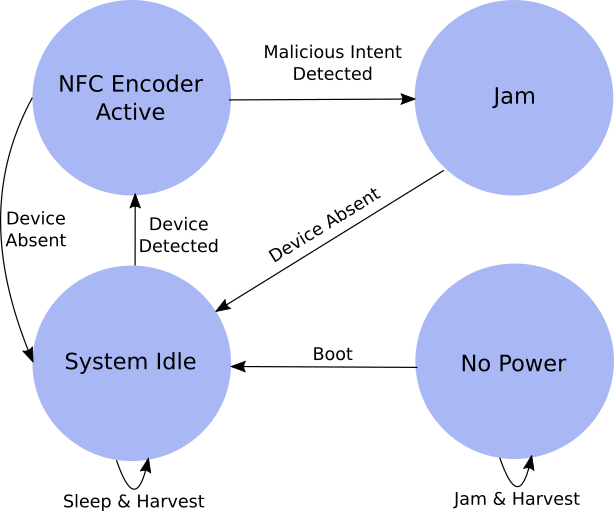
\psfig{file=figures/states.png,width=3in,natwidth=700,natheight=189}
\caption{EnGarde\cite{Gum2013} state digram}
\label{fig:states}
\end{figure}


Commercial payment systems such as Apple Pay and Android Pay are bringing NFC to our phones, which could introduce security risks in both payment and non-payment applications of NFC. This hardware-based firewall may be a viable way to defend against more general threats and it offers flexibility as it reprogrammed address new attacks as they develop. EnGarde is designed to be an extremely power efficient, semi-permanent attachment for everyday mobile phones. Such a device-independent security method, a metaphorical tin foil hat, could protect against current and evolving NFC attacks.~\cite{Gum2013}

Our goal is to give an overview of the EnGarde security system prototyped by Gummeson et al~\cite{Gum2013} in this section. Figure \ref{fig:states} is used as a roadmap for our summary of EnGarde.

\subsection{No Power Mode}

EnGarde is device-independent and is thus not powered directly from the battery contained within the cellphone it is mounted to. Instead, EnGarde contains its own dedicated battery that is charged exclusively by electricity induced into its NFC antenna.\footnote{Power scavenging methods are addressed in great detail in the primary source, but for the this paper, we will not focus how harvesting adequate power from the cellphone works in practice.}
As a result of being independently powered, EnGarde can run on battery and encounter a no-power state. Thus, EnGarde was intentionally designed to fail safe. When EnGarde is in the no power state, it cannot do anything until an NFC signal is detected from either the host phone or an external device. At this point, EnGarde collects power from the NFC signal while simultaneously jamming the ongoing communication. Once enough power is collected, control is handed to the microcontroller.

\subsection{System Idle Mode}
In the system idle state, the microcontroller is running and the EnGarde device simply manages power and waits for an NFC device to move into its vicinity. When an NFC signal is detected, the NFC decoder is activated.

\subsection{NFC Decoder Active Mode}
In this state, we discuss EnGarde's ability to use discretion to block or allow each NFC communication. To do this EnGarde actively scans each transmission from the nearby NFC device in order to determine the other party's intent.

EnGarde is designed to offer real-time protection against malicious attacks from malicious tags, readers, peers, and malicious software. NFC tags can be handy for storing data or URLs in real world applications such as content rich maps or posters. However, such a tag may contain undesirable content, such as a URL to a malicious website. Also, unauthorized NFC readers may attempt to interact with a phone when it is in tag-emulation mode. As a result, location or financial data could be gleaned. Additionally, an NFC phone is ultimately vulnerable to whatever is sent from the peer, since NFC supports file transfers. Finally, a phone owner may inadvertently install malicious software with permission to broadcast via NFC. EnGarde should be able to prevent undesired information sharing over the NFC interface.
\vspace{2mm}\newline
To handle malicious communication, EnGarde scans each message and uses a set of blocking rules to determine if that message should be allowed. The EnGarde is versatile in that current and future undesirable transmissions can be addressed by updating the blocking rules and blacklist.

\subsection{Jam Mode}
When in this mode, EnGarde's goal is to prevent malicious incoming and outgoing communication over NFC. To do this, EnGarde depends on two jamming mechanisms:
\vspace{2mm}\newline
\noindent\textbf{Reflective Jamming:} This defense mechanism is effective against attacks from low-powered tags containing items such as malicious URLs. It works by simply generating a weak signal on the same frequency that the tag is broadcasting to. Since EnGarde is mounted on the back of the owner's phone, EnGarde's signal will be stronger and will effectively block the malicious tag's messages. In additional, the electricity being used to power the tag will also be used to power EnGarde's active defense.
\vspace{2mm}\newline
\noindent\textbf{Pulse Jamming:} If the phone is being attacked by a powered reader or peer device, a much stronger defense, namely generating a competing active transmission, is required to protect the mobile phone. A continuous active transmission would demand far more power then EnGarde could scavenge. Gummeson et al's response is to simply corrupt incoming communication in this case. To corrupt the incoming signal, EnGarde needs to generate a pulse lasting only about 20 microseconds. This brief duration is long enough to corrupt two bits of data, even at the slowest NFC transmission rate.

There is, however, a drawback to the pulse jamming method; a sufficiently high-powered reader could generate a strong enough signal to nullify EnGarde's attempts to corrupt the incoming data. Yet, Gummeson et al counter that an active attack from a high powered reader could be mitigated by using the \textit{reflective jamming} method during the offending reader's discovery protocol. If a connection with a high-powered reader is never established, then EnGarde would not have to use the pulse jamming mechanism against a high-powered reader.

\subsection{Experimental Evaluation of EnGarde}
\noindent\textbf{Jamming:} Both of EnGarde's jamming mechanisms are surprisingly effective. In fact, when Gummeson et al evaluated their device, they found that reflective jamming worked flawlessly against four tags that they tested against. Additionally, they tested the pulse jamming method with general purpose NFC reader and found that EnGarde was able to block 100\% of the responses.
\vspace{2mm}\newline
\noindent\textbf{Decoding:}
Gummeson et al tested EnGarde's decoder using an explicitly defined blacklist set to block all URLs starting with \textit{http://www.malware}. When trying to read tags, one of which contained a blacklisted URL, they found that EnGarde blocked the malicious URL and allowed the benign URL flawlessly.
\vspace{2mm}\newline
Based on these results, it appears that the EnGarde hardware can be very effective at blocking NFC communications it deems malicious. We note, however, that EnGarde's ability to block malicious messages is only as good as its ability to detect them. EnGarde does, however, offer a  programmable, platform independent hardware defense that could certainly be an effective building block for securing NFC as it matures in the future.
\section{Conclusion}
\label{sec:conclusions}

NFC is a young technology and is rapidly growing in popularity due to the deployment of mobile payment system. While the quick setup and ability to communicate with passive tags is attractive, we think that a few hurdles --- specifically security and data transfer speed --- need to be overcome before NFC becomes ubiquitous. In the first study, Jensen, Gouda, and Qiu were able to provide a clever solution to the present security holes by introducing a fortified security scheme for contactless credit cards. While their solution is certainly novel, we discovered that the limited range of NFC is not enough to guarantee security. In the second paper, we reviewed several implementations of mass transit ticketing using NFC on mobile phones. The Nokia researchers were able to provide acceptable solutions given the current state of technology, but have clearly highlighted that the slow data transfer speed of NFC is an obstacle to work around. Finally, Gummeson et al introduced a clever, device independent hardware firewall for NFC on an everyday mobile device. The design of the EnGarde device appears to be incredibly successful at jamming signals, but we note that the protection may only be as good as the firewall rules it uses. Overall, it appears that NFC is a user friendly, flexible communication interface that may become more popular. However, to gain traction, more clever solutions and faster data transfer speeds will be required in order to add sufficient security in the future.

\section*{Acknowledgments}
\label{sec:acknowledgments}

I would like to thank everyone that helped with this project, especially professors Nic McPhee, Elena Machkasova, and Kevin Byod who provided insightful guidance and feedback.

% The following two commands are all you need in the
% initial runs of your .tex file to
% produce the bibliography for the citations in your paper.
\bibliographystyle{abbrv}
% sample_paper.bib is the name of the BibTex file containing the
% bibliography entries. Note that you *don't* include the .bib ending here.
\bibliography{tomSources}
% You must have a proper ".bib" file
%  and remember to run:
% latex bibtex latex latex
% to resolve all references
\end{document}
